\documentclass[10pt]{article}
\usepackage[utf8]{inputenc}
\usepackage{graphicx}
\usepackage{float}
\usepackage{listings}
\usepackage{xcolor}
\usepackage{lmodern}
\usepackage{amsmath}
\usepackage{url}
\graphicspath{{./multi_plant/}}
\lstset{
 basicstyle=\ttfamily,
  columns=fullflexible,
  frame=single,
  breaklines=true,
  postbreak=\mbox{\textcolor{red}{$\hookrightarrow$}\space},
}
\linespread{1.1}
\title{\Large Plant segmentation and labeling}
\author{Kacper Reja}
\date{}

\begin{document}

\maketitle

\tableofcontents
\clearpage
\section{Introduction}
The goal of our task was to perform leaf segmentation from given multi-view dataset containing high resolution images of plants captured with three fixed cameras. More precisely we had to segment provided pictures such that each leaf was labeled with different color so we could easily distinct them.
\begin{figure}[H]
\caption{Sample of input images}
\includegraphics[width=0.5\textwidth]{rgb_00_00_000_00}
\includegraphics[width=0.5\textwidth]{rgb_00_00_003_00}
\includegraphics[width=0.5\textwidth]{rgb_00_00_006_00}
\includegraphics[width=0.5\textwidth]{rgb_00_00_009_00}
\end{figure}

Photos of each plant were taken six times a day for ten days. There were five plants and three cameras.
\clearpage
\section{Algorithm description}
In this project the Watershed Algorithm approach was used to segment images. The script was built mostly based on observation that all plants were in some tone of green color and the background was mainly white. This knowledge was used to create our grayscale image using inRange function with manually chosen color values to fit the best. 
\begin{lstlisting}[language=Python]
#convert to hsv and inRange
hsv = cv2.cvtColor(img, cv2.COLOR_BGR2HSV)
#range choosen manually with help of a colorpicker to highlight green color
green = cv2.inRange(hsv, (20,37,30), (70,140,106))
\end{lstlisting}
\begin{figure}[H]
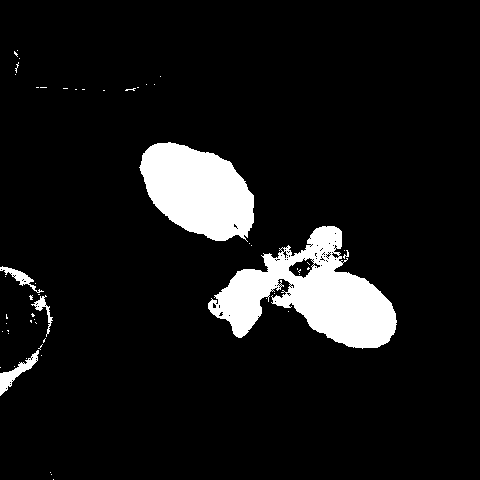
\includegraphics[width=\textwidth]{../example/grayscale}
\end{figure}
\clearpage
After that we perform noise removal to clean up the background a bit
\begin{lstlisting}[language=Python]
#noise removal
kernel = numpy.ones((3,3), numpy.uint8)
opening = cv2.morphologyEx(green,cv2.MORPH_OPEN,kernel)
\end{lstlisting}

\begin{figure}[H]
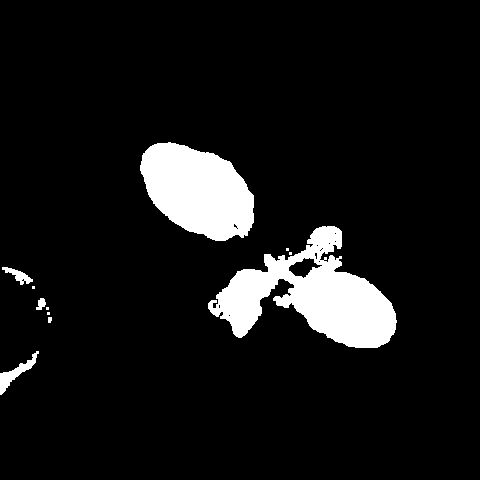
\includegraphics[width=\textwidth]{../example/grayscale_clean}
\end{figure}

\clearpage
Next we have to extract the area which we are sure they are leaves. Since leaves might be touching each other, we use the distance transform and apply a proper threshold. We also have to find the area which we are sure they are not leaves. We use dilation which increases object boundary to background.
\begin{lstlisting}[language=Python]
#sure background area
sure_bg = cv2.dilate(opening,kernel, iterations = 8)
#sure foreground area using Distance Transformation
dist_transform = cv2.distanceTransform(opening, cv2.DIST_C, 3)
(ret, sure_fg) = cv2.threshold(dist_transform, 0.15*dist_transform.max(), 255, 0)
\end{lstlisting}

\begin{figure}[H]
\caption{Sure foreground}
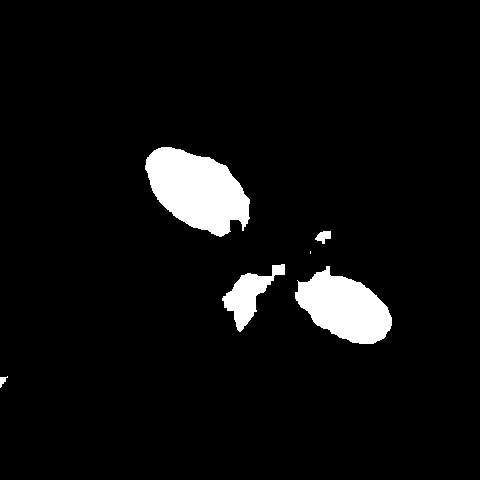
\includegraphics[width=\textwidth]{../example/sure_fg}
\end{figure}
\begin{figure}[H]
\caption{Sure background}
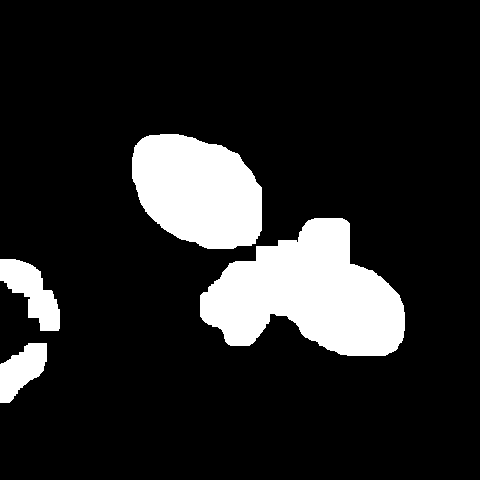
\includegraphics[width=\textwidth]{../example/sure_bg}
\end{figure}
\clearpage
After that we can obtain unknown region by substracting sure foreground area from sure background area.
\begin{lstlisting}[language=Python]
#finding unknown region
sure_fg = numpy.uint8(sure_fg)
unknown = cv2.subtract(sure_bg, sure_fg)
\end{lstlisting}
\begin{figure}[H]
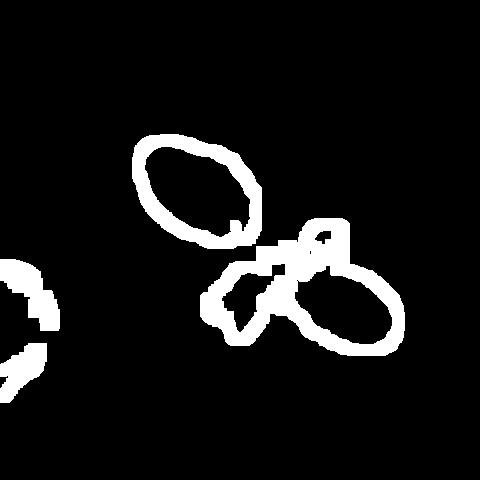
\includegraphics[width=\textwidth]{../example/unknown}
\end{figure}
\clearpage
Now that we know for sure which are region of leaves and which are background we can create marker and label those regions. After that we can use watershed algorithm.
\begin{lstlisting}[language=Python]
#marker labelling
(ret, markers) = cv2.connectedComponents(sure_fg)
#add one to all labels so that sure background is not 0 but 1 so that watershed algorithm won't consider it as unknown area
markers = markers + 1
#now mark the region of unknown with zero
markers[unknown==255] = 0
#perform watershed algorithm
markers = cv2.watershed(img,markers)
\end{lstlisting}
\begin{figure}[H]
\caption{Marker image}
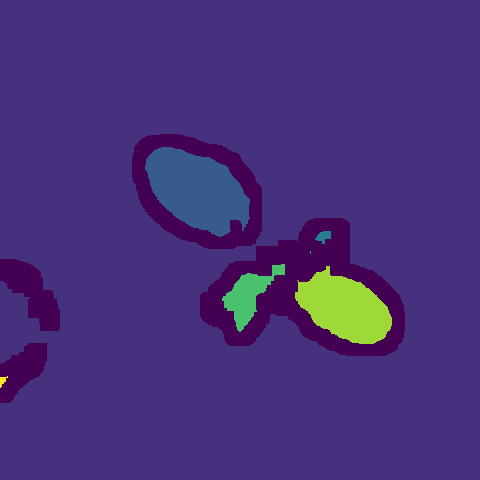
\includegraphics[width=\textwidth]{../example/markers}
\end{figure}
\begin{figure}[H]
\caption{Marker image after segmentation}
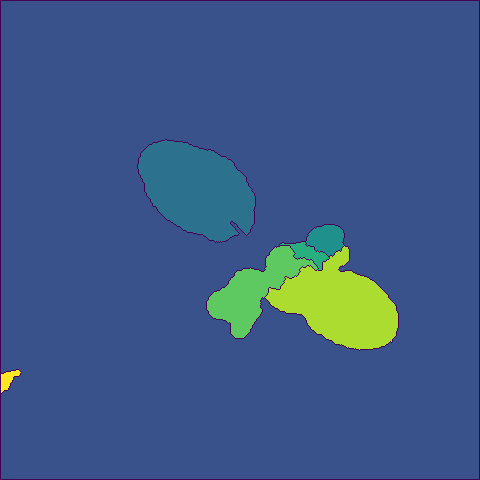
\includegraphics[width=\textwidth]{../example/segmented}
\end{figure}
\section{Results}
To check accuracy of the script dice similarity coefficient was used. Even though trying to get the best results with different hsv values when creating grayscale image and optimizing noise removal, finding sure background and foreground areas only 82\% accuracy was obtained which definitely leaves a lot to be desired. We can see in example given above that leaves were merging and stem might not be recognized. Biggest problems when separating leaves from background were plant pot which was visible under leaves and the fact that some leaves were lighted with different amounts of light.
\clearpage
\section{Source code}

\begin{lstlisting}[language=Python]
#Watershed algorithm
#import the necessary packages
import cv2
import numpy
import matplotlib.pyplot as plt
import os
#load the color image 
sourcepath = 'multi_plant/'
outputpath = 'result_label/'
gtpath =  'multi_label/'
maskpath = 'mask_result/'
if not os.path.exists(sourcepath):
    print('Path' + sourcepath + 'does not exist')
    exit(1)
if not os.path.exists(outputpath):
    print('Path' + outputpath + 'does not exist')
    exit(1)
if not os.path.exists(gtpath):
    print('Path' + gtpath + 'does not exist')
    exit(1)
dices = []
a=0 #camera id
b=0 #plant id
c=0 #day id
d=0 #time id
for i in range (0, 900):

    imageName = f'rgb_0{a}_0{b}_00{c}_0{d}'
    labelName = f'label_0{a}_0{b}_00{c}_0{d}'
    d=d+1
    if d>5:
        d=0
        c=c+1
    if c>9:
        c=0
        b=b+1
    if b>4:
        b=0
        a=a+1     


    #read image and ground truth label
    img = cv2.imread(sourcepath + imageName + '.png' , cv2.IMREAD_COLOR)
    label = cv2.imread(gtpath + labelName + '.png', cv2.IMREAD_COLOR)
    
    #convert to hsv and inRange
    hsv = cv2.cvtColor(img, cv2.COLOR_BGR2HSV)
    #range choosen manually with help of a colorpicker to highlight green color
    green = cv2.inRange(hsv, (20,37,30), (70,140,106))

    #noise removal
    kernel = numpy.ones((3,3), numpy.uint8)
    opening = cv2.morphologyEx(green,cv2.MORPH_OPEN,kernel)

    #sure background area
    sure_bg = cv2.dilate(opening,kernel, iterations = 8)

    #sure foreground area using Distance Transformation
    dist_transform = cv2.distanceTransform(opening, cv2.DIST_C, 3)
    (ret, sure_fg) = cv2.threshold(dist_transform, 0.15*dist_transform.max(), 255, 0)

    #finding unknown region
    sure_fg = numpy.uint8(sure_fg)
    unknown = cv2.subtract(sure_bg, sure_fg)

    #marker labelling
    (ret, markers) = cv2.connectedComponents(sure_fg)

    #add one to all labels so that sure background is not 0 but 1 so that watershed algorithm won't consider it as unknown area
    markers = markers + 1

    #now mark the region of unknown with zero
    markers[unknown==255] = 0
    #perform watershed algorithm
    markers = cv2.watershed(img,markers)
    
    #saving to result folder
    plt.imshow(markers)
    plt.imsave(outputpath + imageName + '_segmented' + '.png', markers)

    #invert color of markers
    markers[markers==1] = 255
    markers= 255 - markers

    #saving mask result
    cv2.imwrite(maskpath + imageName + '_mask' + '.png', markers)
    

    #dice similarity
    label = cv2.cvtColor(label, cv2.COLOR_BGR2GRAY)
    (thresh1, gt) = cv2.threshold(label, 1, 255, cv2.THRESH_BINARY)

    res = cv2.imread(maskpath + imageName + '_mask' + '.png')
    res = cv2.cvtColor(res, cv2.COLOR_BGR2GRAY)
    (thresh2, seg) = cv2.threshold(res, 1, 255, cv2.THRESH_BINARY)


    k=255

    dice = numpy.sum(seg[gt==k])*2.0 / (numpy.sum(seg) + numpy.sum(gt))
    dices.append(dice)

    #end of for loop
print('mean dice sim score {}'.format(numpy.mean(dices)))
\end{lstlisting}
\clearpage
\begin{thebibliography}{9}
\bibitem{1}
\url{https://docs.opencv.org/master/d3/db4/tutorial_py_watershed.html}

\bibitem{2}
\url{https://docs.opencv.org/trunk/d7/d1c/tutorial_js_watershed.html}

\bibitem{3}
\url{https://en.wikipedia.org/wiki/S\%C3\%B8rensen\%E2\%80\%93Dice_coefficient}

\bibitem{4}
\url{https://en.wikipedia.org/wiki/Watershed_(image_processing)}
\end{thebibliography}

\end{document}